\documentclass[12pt]{article}%%
%\usepackage{enstyle}  % Loads my formatting
%\usepackage{stata}
%\usepackage{etoolbox}
\usepackage{amssymb}
\usepackage{amsmath,bm} % 数学符号公式统一加粗 \bm{}
\usepackage{amsfonts}
\usepackage{amsmath}
\usepackage[nohead]{geometry}
\usepackage[singlespacing]{setspace}
\usepackage[bottom]{footmisc}
\usepackage{indentfirst}
\usepackage{endnotes}
\usepackage{graphicx}%
\usepackage{subfigure}
\usepackage{rotating}
\usepackage[colorlinks=true]{hyperref}
\usepackage{longtable}
\usepackage{dcolumn}
\usepackage{rotating}
\usepackage{booktabs}
\usepackage{harvard}
\usepackage{CJK}
\usepackage{indentfirst} %使首段段首也缩进
\usepackage{lscape} %使某一页横排,但只有在postscript 或PDF文件中才能看到正确的效果。
\usepackage{ragged2e} %两端对齐
\justifying\let\raggedright\justifying
\setcounter{MaxMatrixCols}{30}
\newtheorem{theorem}{Theorem}
\newtheorem{acknowledgement}{Acknowledgement}
\newtheorem{algorithm}[theorem]{Algorithm}
\newtheorem{axiom}[theorem]{Axiom}
\newtheorem{case}[theorem]{Case}
\newtheorem{claim}[theorem]{Claim}
\newtheorem{conclusion}[theorem]{Conclusion}
\newtheorem{condition}[theorem]{Condition}
\newtheorem{conjecture}[theorem]{Conjecture}
\newtheorem{corollary}[theorem]{Corollary}
\newtheorem{criterion}[theorem]{Criterion}
\newtheorem{definition}[theorem]{Definition}
\newtheorem{example}[theorem]{Example}
\newtheorem{exercise}[theorem]{Exercise}
\newtheorem{lemma}[theorem]{Lemma}
\newtheorem{notation}[theorem]{Notation}
\newtheorem{problem}[theorem]{Problem}
\newtheorem{proposition}{Proposition}
\newtheorem{remark}[theorem]{Remark}
\newtheorem{solution}[theorem]{Solution}
\newtheorem{summary}[theorem]{Summary}
\newenvironment{proof}[1][Proof]{\noindent\textbf{#1.} }{\ \rule{0.5em}{0.5em}}
\makeatletter
\def\@biblabel#1{\hspace*{-\labelsep}}
\makeatother
\geometry{left=1in,right=1in,top=1.00in,bottom=1.0in}
\begin{document}

\begin{CJK*}{GBK}{fs}
%繁体字库:GB, Big5
%%%%%%%%%%%%%%%%%%%%%%%%%%%%%%%%%%%%%%%%%%%%%%%%%%%%%%%%%%%%%%%%%%%%%%%%%%%%%%%

\title{Vertical Spillover of Innovation and Firm Performance: Evidence from China\footnote{Preliminary} \\
\quad \quad \quad \quad \quad \quad \quad \quad \quad \quad \quad \quad \quad \quad
%Quality \emph{or} Quantity? \\
%\hfill {\Large  Evidence from Chinese Patents Data}
}
\sloppy%
%\onehalfspacing

%\author{Yang Shen \thanks{Yang Shen, School of Economics, Fudan University, Student ID: 18110680011}}
\author{Qisheng Cai\thanks{Qisheng Cai, School of Business, Shanghai University of Finance and Economics} \ Yang Shen \thanks{Yang Shen, China Centre for Economic Studies, School of Economics, Fudan University} \ Zhengyu Yuan\thanks{Zhengyu Yuan, Institute of World Economy, School of Economics, Fudan University}}

\date{2018-11}
\maketitle
\sloppy%
\onehalfspacing
\textbf{Abstract}
Innovation is seen as a fundamental source for the growth of economy and companies. We investigate how technology spillovers through input-output linkages impact firms' productivity. After combining patent application data and detailed firm-level survey, the empirical results show that a one standard-deviation increase of knowledge spillovers from upstream will lead to a 0.5\% TFP growth while the downstream spillovers only impact firms facing credit constraint. Additionally, the gains from upstream knowledge spillovers strongly benefit firms with lower initial productivity, more downstreamness and in high-tech sectors. Our findings emphasize the importance of vertical knowledge spillovers for economic growth especially when facing financial frictions.   \\
\textbf{Keywords:}
Vertical Spillovers; Productivity; Patent; Credit Constraints \\
\textbf{JEL Classification Numbers:} O31, D24, D57
\thispagestyle{empty}
\pagebreak%

%\underline{\textbf{Non-technical summary}}
%\begin{enumerate}
%  \item
%  \item
%  \item
%  \item
%  \item
%  \item
%  \item
% \end{enumerate}
%\thispagestyle{empty}
%\pagebreak%
%\doublespacing

\newpage



\section{INTRODUCTION}
 After a long-term growth miracle over past decades, China has started to attach great importance on the power of innovation and invested heavily in research in the past years instead of relying on cheap labor force and low-efficient investment(\textcolor[rgb]{0.00,0.07,1.00}{Wei~et~al.(2017)}), by which, the surge of China's patenting applications has aroused great notice over the world. In the year of 2011, China has overtook the U.S. and became the NO.1 economy all over the world who has most resident patent application(\textcolor[rgb]{0.00,0.07,1.00}{Albert~et~al.(2016)}). Existing studies have proven the positive and significant effect of patent on firm's TFP(\textcolor[rgb]{0.00,0.07,1.00}{Bloom \& Van Reenen (2002)},\textcolor[rgb]{0.00,0.07,1.00}{Albert~et~al.(2016)}). However, most studies only pay close attention to the innovation within firms, whereas ignore the important effect of knowledge spillover. Combining patent application data from State Intellectual Property Office(SIPO) and Annual Survey of Industrial Firms, our paper fills the gap of literatures by examining the knowledge spillover effect of innovation on productivity, especially from the perspective of vertical spillover. Because of the law of patent protection and competition effect, the horizontal spillovers within the same industry could be restricted to a large extent or even be negative for small firms, while the spillover from upstream could be received intermediately(since there is lower possibility for inter-sector imitation) and our empirical result shows that a one standard-deviation increase of knowledge spillovers from upstream will lead to 0.5\% TFP growth. The effect is very similar when we use the total patent application or more reliably, the number of invention patent application and citation with 5-year cohort. This is also valid when we control firm size, registration type, and spillovers within the same sectors.  \par
 Moreover, though the existing papers show that financial development is an important advantage for trade and firms in sectors facing less credit constraints have better export performance(\textcolor[rgb]{0.00,0.07,1.00}{Manova(2013)},\textcolor[rgb]{0.00,0.07,1.00}{Manova~et~al.(2015)}), we show that firms facing credit constrains could gain more from vertical knowledge spillovers. Specifically, a one standard deviation increase in knowledge spillovers from upstream will improve firm's TFP in the sector at the 75th percentile of the distribution by inventory ratio by 14.4\% more than in the sector at the 25th percentile and 19.8\% less when it comes to asset tangibility.  Because firms in sectors with more credit constraints rely on vertical spillovers much more seriously, which need little fixed costs but a lower marginal input prices and higher input quality. However, our result does not mean that financial frictions are better for firm absorbing vertical spillovers, but to indicate another channel which companies could improve their production efficiencies. Since innovation is the output of R\&D, firms with higher asset tangibility or lower inventory to sales ratio do research and innovate much easier where the refining in upstream provide little to TFP. \par
 We also uses series of robustness checks to explore the various impacts of heterogeneity among sectors and firms. Low technic sectors gains more from vertical knowledge spillovers. The effect is both significant for sectors in upstream and downstream and firms with size at the top 5th percentile could get more benefit than medium and small size firms.  We also establish that local firms can transform more vertical knowledge spillovers into TFP, while the effect is not significant for foreign enterprises registered by Hong Kong, Macao and Taiwan regions of China. At last, we use the lagged variable as instrument to support our main findings.  \par
The rest of the paper is organised as follows. Section 2 gives a overview of existing literatures. Section 3 introduce the data we use. Section 4 shows the empirical strategies and benchmark results. Section 5 is the robustness checks and section 6 concludes.


\section{RELATED LITERATURE}
Our paper relates to several aspects of literatures.In the first strand, many papers have examined the relationship between innovation and growth of productivity. A majority of empirical studies find that innovation contributed significantly to productivity growth. \textcolor[rgb]{0.00,0.07,1.00}{Griliches(1998)} find evidence of a direct R\&D impact on productivity. \textcolor[rgb]{0.00,0.07,1.00}{Hig\'{o}n(2007)} indicates that R\&D efforts have a positive impact on the industry's productivity.   \textcolor[rgb]{0.00,0.07,1.00}{Cui \& Li(2016)} uses the U.S. manufacturers' patent data and find that productivity is positively correlated with the number of patents granted, the number of technological categories for these patents and the number of citations per granted patent. The same pattern has been found in \textcolor[rgb]{0.00,0.07,1.00}{Albert~et~al.(2016)}, who uses Chinese patent application data to explain the phenomenon of patent surge in 2007-2011. Though they find a positive relationship between patent number and R\&D and productivity, the trend seems to be weaker as time goes, which may support the government policy incentive hypothesis. Some papers focus on the foreign R\&D capital diffusion and they find while foreign R\&D has beneficial effects on domestic productivity(\textcolor[rgb]{0.00,0.07,1.00}{Coe \& Helpman,1995; Guellec \& De La Potterie,2002}).\par
A large body of literatures investigate other factors having effects on the transformation from innovation to TFP. Especially, financial conditions would restrict innovation input, which then affect firm's TFP. \textcolor[rgb]{0.00,0.07,1.00}{Himmelberg \& Petersen(1994)} suggest that the flow of internal finance is the principal determinant of R\&D investment. \textcolor[rgb]{0.00,0.07,1.00}{Aghion et al.(2012)} shows that in more credit-constrained firms, R\&D investment plummets during recessions but does not increase proportionally during upturns, and productivity growth are more negatively correlated with sales volatility. \textcolor[rgb]{0.00,0.07,1.00}{Hottenrott \& Peters,(2012)} find that firms with high innovative capability and low levels of internal funds are more likely to be constrained than their more liquid counterparts.  \par
The second strand of literatures refer to spillover effects through input-output linkages. Several papers verify that a positive shock can be propagated through input-ouput linkages which firms can be benefited from. \textcolor[rgb]{0.00,0.07,1.00}{Javorcik(2004)} demonstrates the importance of upstream and downstream linkages as channels for FDI to have positive effects on domestic firms. \textcolor[rgb]{0.00,0.07,1.00}{Lu et al.(2017)} find FDI in the same industry hurts the productivity of domestic firms while the effects of both backward and forward FDI on firm productivity are positive. With respect to innovation spillover through input-ouput linkage, \textcolor[rgb]{0.00,0.07,1.00}{ Atallah(2002)} studies vertical R\&D spillovers between upstream and downstream firms, who find that vertical spillovers always increase R\&D and welfare, while the effect of horizontal spillovers is ambiguous. \textcolor[rgb]{0.00,0.07,1.00}{Acemoglu et al.(2015)} find substantial propagation of foreign patenting shocks through the input-output network, and the network-based propagation is larger than the direct effects of the shocks. On the other hand, firm's financial condition is a key factor which can affect the spillover process to firms. \textcolor[rgb]{0.00,0.07,1.00}{Alfaro et al.(2004)} develops the idea that better financial conditions allow agents to take advantage of spillovers from foreign investment. \textcolor[rgb]{0.00,0.07,1.00}{Agarwal et al.(2014)} find that credit constraints affect Chinese firms' absorption of productivity spillovers originating from foreign-owned firms. \par
Unlike the prior work, \textcolor[rgb]{0.00,0.07,1.00}{Bernard et al.(2018)} use detailed firm-to-firm data to unlock the "black box" of productivity dispersion among firms. From a network perspective, they find that firms can be larger because of more buyers and well-matched buyers which mentioned as "downstream effect", or firm can benefit from own production capability leading to supplier capability well-matched suppliers through "upstream effect". Moreover, the downstream factors explain the vast majority of firm size dispersion. \par
At last, our paper also links to literature studying the role of credit constraints on firm performance. \textcolor[rgb]{0.00,0.07,1.00}{Manova(2013)} incorporate financial frictions into heterogeneity-firm-export model and shows that credit constraints enhance the "selection effects" both intensively and extensively. While developed countries have a comparative exporting advantage in financially vulnerable sectors, developing countries are suffering from the unhealthy financial system. Moreover, while financial frictions deeply restrict firms' export, \textcolor[rgb]{0.00,0.07,1.00}{Manova~et~al.(2015)} suggest that firms can easy access to foreign capital have a comparative advantage at sectors financially vulnerable, which refers to MNCs whose parent company can directly fund their affiliates and joint ventures. Similarly, since international trade relies much more on outside capital in case of upfront costs and higher economic risk, which are much more important for ordinary trade than processing trade since the former need more working capital for higher up-front costs. \textcolor[rgb]{0.00,0.07,1.00}{Manova \& Yu(2016)} indicates that credit constraints restrict Chinese firms to less profitable activities, on the other words, processing trade. However, processing trade do not hurt Chinese export but allows firms dependent on external finance to participate in global value chains and share the gains from trade.


\section{DATA DESCRIPTION}
\subsection{TFP and Innovation}
Our empirical analysis combines three data sets. The first data set is China State Intellectual Property Office(SIPO) Patent Database (1998-2007), which contains application number, applicant, application type(domestic or abroad), and 4-digit IPC classification. According to the concordance between IPC code and China National economic industry classification (CIC) from the State Intellectual Property Office, we compute the number of patents within every industry-year pair of three types: invention, utility and foreign. We drop the design patens because it does not contribute to the firm productivity growth. Figure 1 plots the trend of these three patent type, the total number of patent application is increasing at the rate of 4.9\%, and 3.0\%, 0.84\%, 0.76\% for invention, utility and foreign patent application respectively. The invention patent application has seen a surge after the year of 2002, when China entered WTO and been access to a large variety of high-tech imports abroad. The foreign patent application also grew faster after 2000.    \par
\begin{center}
  [Insert Figure 1 here]
\end{center}
\par Our second data set is Annual Survey of Industrial Firms (ASIF) (1998-2007) which includes all state-owned enterprises and non-SOE enterprises with annual sales over 5 million RMB. We get the information of firm annual output, employment, capital, ownership and also their industry code.\footnote{\scriptsize The CIC code has been changed after the year of 2002. We adjust the industry code after 2002 and make it consistent with pre-2002.} We adopt the same method with \textcolor[rgb]{0.00,0.07,1.00}{Manova~et~al.(2015)} droping the SOE observations since they are not necessarily profit-maximizing entities.\par
The third data set is China detailed input-output table (2002), which contains 122 input-output sector including agriculture, manufacture and service industries. We use the 2002 version because it is more representative through our data set than the 2007 version. And the input-output relationship between sectors is quite state between 2002 and 2007(\textcolor[rgb]{0.00,0.07,1.00}{Ju \& Yu(2015)}). The concordance table between I-O code and CIC code is from Brandt. Table 1 shows the description statistics.
\begin{center}
  [Insert Table 1 here]
\end{center}


\subsection{Credit Constraints}
We use \emph{External financial dependence} to measure financial vulnerable for each sector. The data is coming from \textcolor[rgb]{0.00,0.07,1.00}{Manova~et~al.(2015)} which is constructed by the share of capital expenditures not financed out of cash flows from operations. It is the median level US-firms for each sector relying on the outside capital and describes the technical factor for each industry, which is quite stable across time(\textcolor[rgb]{0.00,0.07,1.00}{Manova,2013; Manova~et~al.,2015}). Another advantage is that this index is calculated by the US data and is proved to be common for firms all over the world, and more importantly, exogenous for China(\textcolor[rgb]{0.00,0.07,1.00}{Chen~et~al.,2017}). \par
Typically there is also another index often used in literature, \emph{Asset Tangibility}, measuring the ability to raise external finance by pledging the available tangible assets used in production(such as plants and equipment) as collateral. We have two concerns why \emph{Asset Tangibility} may not be suitable for this paper. The first is that \emph{External financial dependence} pointing directly to long-term investment such as $R\&D$ and innovated investment, which is exactly what we want to mention here. \emph{Asset Tangibility}, however, is much more general since it measures the whole ability firms can pledging hard and tangible assets as collateral. Therefore it is too mixed to infer to innovation. The second concern is that although a non-state-owned firm have enough tangible assets(plant,equipments), it could still be constrained by the inefficient State-favored system of China's banking sector (\textcolor[rgb]{0.00,0.07,1.00}{Dollar \& Wei,2007; Chen~et~al.,2017}). \textcolor[rgb]{0.00,0.07,1.00}{Wu(2018)} finds that 70\% aggregate TFP loss is due to policy distortions in China since state-owned firms' low capital constraints. Similarly, \textcolor[rgb]{0.00,0.07,1.00}{Dollar \& Wei,(2007)} suggests that if the policy-induced liquidity constraint faced by private firms could be fixed, China will get an additional 5 percentage GDP. And \textcolor[rgb]{0.00,0.07,1.00}{Hsieh \& Klenow,(2009)} illustrates that China would get 30\%-50\% manufacture TFP gains if reallocate the capital to the level of the U.S.. Both of the information mentioned above makes \emph{Asset Tangibility} not suitable for measuring access to outside capital of non-SOEs in China, especially for innovative investment.

\section{EMPIRICAL ANANLYSIS}
\subsection{EMPIRICAL DESIGN}
Our first specification is to study how knowledge spillovers impact the firm productivity through vertical linkage:
\begin{equation}
  \ln TFP_{fjt}=\alpha+\beta_1 Vertical\_spillover_{jt}^{up}+\beta_2 Vertical\_spillover_{jt}^{down}+\gamma X_{fjt}+\lambda_{j}+\eta_{t}+\phi_{f}+\epsilon_{fjt}
\end{equation}
where $\ln TFP_{fjt}$ represents $TFP$ of firm $f$ in industry$j$. $Vertical\_spillover_{jt}^{up}$ denotes the knowledge spillovers from $j$'s upstream, which is the weighted average of patent application:
\begin{equation*}
  Vertical\_spillover_{jt}^{up,D}=\sum\limits_k\frac{input_{kj}}{\sum_{i}input_{ij}} \cdot \ln patent_{kt}
\end{equation*}
where the numerator in the weight denotes the input from sector $k$ to $j$, whereas the denominator is all intermediate inputs used by sector $j$. Thus the weight computes the inputs from sector $k$ when produce one amount of product $j$. $\ln patent_{kt}$ is the patent application number of sector $k$. Therefore, it measures the magnitude of knowledge spillover from upstream of sector $j$. Note that it measures the direct sector-to-sector knowledge spillover which counts the first-order spillover effect and ignores the cycling in input-output table. To describe the full chain relationship, we instead use the following specification:
\begin{equation*}
  Vertical\_spillover_{jt}^{up,L}=(I-\Omega)^{-1}\cdot \ln patent_{kt}
\end{equation*}
where $(I-\Omega)^{-1}=\sum I+\Omega+\Omega^2+...$ is the Leontief inverse matrix which accounts the full chain linkages. $\Omega$ is the matrix of $\omega_{kj}^{up}=\frac{input_{kj}}{\sum_{i}input_{ij}}$.  The construction of downstream knowledge spillover is similar with $Vertical\_spillover_{jt}^{up}$:
\begin{equation*}
  Vertical\_spillover_{jt}^{down,D}=\sum\limits_g\frac{input_{jg}}{\sum_{i}input_{ji}} \cdot \ln patent_{gt}
\end{equation*}
It is the weighted average of downstream patents where the weight reflects how much intermediate goods sector $g$ need to produce one value good from sector $j$. We will also use the Leontief inverse matrix to cover the full chain aspects, that is,  $Vertical\_spillover_{jt}^{down,L}$. \par
One problem to use patent application number mirroring innovation capacity is the great difference between patent quality. A usual method is to use citation of each patent, where higher citation means more agencies adopt the innovation. In 1998, the citation of each IPC code varies from 0 to 3624. However, since patents applicated later are less likely to be cited than earlier one, we also use the 5-year citation cohort for each patent. For instance, we count the citation record between 2000 and 2004 for patent applied in 2000. Because the last year of our sample is 2007, we will end the statistics in 2011\footnote{\scriptsize The SIPO database updates every record of citation for each patent.}. \par

$X_{ijt}$ is a vector of time-varying firm controls which includes sector patent application number, firm size(logarithm of firm total output) and a dummy variable for foreign firm. Bigger firms usually have higher productivity while foreign firms have lower TFPs than private firms on average. We use sector patent application number to control horizontal spillover effects within sector. $\lambda_{j}$ is sector fixed effect, $\eta_{t}$ is year fixed effect and $\phi_{f}$ is firm fixed effect. In case of the serial correlation problem, standard errors are clustered at sector level.
\par
To access different patterns that firms take advantage of knowledge spillovers when facing financial constrain, we estimate the following model:
\begin{align}
   \ln TFP_{fjt}= & \alpha+\beta_1 Vertical\_spillover_{jt}^{up}+\beta_2 Vertical\_spillover_{jt}^{down} \notag  \\
      +\beta_3    &  Vertical\_spillover_{jt}^{down} \times FinVuln_j+\lambda X_{fjt}+\lambda_{j}+\eta_{t}+\phi_{f}+\epsilon_{fjt}
\end{align}

where $FinVuln_j$ is \emph{External financial dependence} across sectors and time-invariant. The interaction between $Vertical\_spillover_{jt}^{up}$ and $FinVuln_j$ capture how firm transforms the innovation from upstream into production when facing different financial constrains. Similarly, the interaction between $Vertical\_spillover_{jt}^{down}$ and $FinVuln_j$ capture how firm benefits from improvements of their customers when hard access to outside capital. Firms will get gains from lower marginal costs of intermediate goods and interacting with better customers. Both benefits could probably be much important for firms facing credit constraints who relying much on external finance, since firms could manage when and how to innovate without waiting for the technology shock from upstream or downstream. \par


\subsection{MAIN RESULTS}
Table 2 is the regression result for model $(1)$ and uses patent applications to measure vertical knowledge spillovers. Column (1)-(4) only calculate the direct sector linkage while column (5)-(8) include the full chain effect by Leontief inverse matrix. All regressions have added firm fixed effects to control all unobservable factors influence firm's TFP and sector and year fixed effects to control common macro shock for each sector and all firms in a given year.  Upstream spillovers are all positive and significant at 5\% or 1\% level, which means that the innovation by suppliers either decreasing the input costs or increasing the quality of intermediate goods. However, after we control firm size and foreign firm dummy, the effect of downstream spillovers disappeared, which indicates that firms would not be benefited from better customers averagely. Quantitatively, a one standard-deviation increase of knowledge spillovers from upstream will lead to a 0.374\% TFP growth indicated in column (4) and 0.675\% in column (8), which is doubled when considering the full chain effect. Firm size has positive impact on TFP and foreign firm is lower efficient than private firm. Spillovers from the same sector has statistically negative impact on TFP. It may be the reason that the innovation from others from same sector crows out the market share and hurt other firms' profit and productivity for innovation is winner-takes-all game. \par
Table 3 gives the similar empirical results for model $(1)$ except for using citation with 5-year cohort to reflect the quality of innovation. The effect of knowledge spillovers from upstream remains significantly positive, and a one standard-deviation increase of knowledge spillovers from upstream will lead to a 0.475\% TFP growth from column (8). Firms take no advantage from innovation in downstream.

\begin{center}
  [Insert Table 2 here]
\end{center}
\begin{center}
  [Insert Table 3 here]
\end{center}

\par  Table 4 shows the empirical results for model (2) by adding the interaction between vertical knowledge spillovers both from upstream and downstream, where column (1)-(3) measure the direct vertical spillovers and column (4)-(6) calculate it by Leontief inverse matrix. The coefficients of upstream spillover are still significantly positive and downstream spillover are not significant. However, after we control firm size and indicator for foreign firm, the interaction between downstream spillovers and \emph{External financial dependence} is positive and significant whether we use the direct linkage or full chain effect while interaction between upstream spillovers and \emph{External financial dependence} is not significant at all. These differential results shows that though all firms could benefit from the lower marginal costs or higher quality from suppliers, only those facing credit constraints will be improved by technological progress from downstream. The explanation is that while everyone could get gains from better intermediated goods or higher capacity of their suppliers, improvements of customers will only impact firms who make R\&D inefficiently since others access to outside capital easily have already got the technical frontier. In case to be abandoned, firms will raise the productivity to meet the higher demand, which can not threat firms having enough capital to do long-term investment, like R\&D. Specifically, column (3) shows that a one-standard deviation increase in knowledge spillovers from downstream will improve firm's TFP in the sector at the 75th percentile of the distribution by \emph{External financial dependence} by 0.15\% more than in the sector at the 25th percentile. When come to the full chain effect, column (6) shows that the effect is 0.05\% more at the 75th percentile than the 25th percentile. We replace patent application number with citation in table 5 for a more accurate result. The quantitative implication is that a one-standard deviation increase in knowledge spillovers from downstream will be 0.2\% more for sectors at the 75th percentile of the distribution by \emph{External financial dependence} than sectors at 25th percentile, which is bigger than considering the full chain effect where is 0.08\%\footnote{\scriptsize The reason why the full chain effect is smaller than the direct linkage is that the mean of the former is 3 times more than the latter one, which means that the economic implication is very similar for the two measurements.}.
\begin{center}
  [Insert Table 4 here]
\end{center}
\begin{center}
  [Insert Table 5 here]
\end{center}



\section{ROBUSTNESS CHECK}
We address several mechanisms in this section to examine the robustness of our core findings. First we use invention patent instead of all types of patent. Second, we detect the ability firm can absorb knowledge spillovers conditional on heterogeneity of sector and firm size. Then we show more valid evidences for model 2.


\subsection{INVENTION PATENT}
As illustrated above, the quality of patent varies a lot, especially comparing invention patent and utility patent. Invention patents need significant progress compared to prior technology while utility patent only need new technical solution for the shape, construction of products. Apparently invention patent worth much more than utility patent in the technical aspect. Moreover, there is a much stricter review progress for invention patent which lasts more than a year. However, utility patent only takes a half of year and will not be rejected mostly. Thus, the number of invention patent could be a more precise standard for innovation quality. In consideration of the unreliable application of utility patents, we replace the total patent application with invention patent for a more logical measure. Table 6 indicates that a one standard-deviation increase of weighted sum of invention patent from upstream lead to 1.49\% and 3.9\% TFP growth averagely by column (1) and (3) respectively, much higher comparing with the benchmark results by table 2. When considering financial vulnerable, the spillover effects of downstream is 0.12\% and 0.04\% stronger for sectors at the 75th percentile than the 25th percentile by the distribution of \emph{External financial dependence} for direct linkage and full chain effects respectively.
\begin{center}
  [Insert Table 6 here]
\end{center}

\subsection{FIRM HETEROGENEITY}
\par The absorptive capacity for vertical knowledge spillovers mat vary at several dimensions. We emphasize two important aspects in this section. First the different ways of sourcing and financing ability make private firms more dependent on vertical spillovers than foreign firms where the latter can access foreign capital markets or funding from
their parent company(\textcolor[rgb]{0.00,0.07,1.00}{Monova~et~al.,2015}). Table 7 gives the evidence for firms with different types respectively, where column (1) and (3) only includes private firms and column (2) and (4) are all foreign firms. Vertical Knowledge spillovers are built by citation in 5-year cohort. It is clear that upstream knowledge spillovers could raise both private and foreign firms' productivity performance(the p-value of $up\_spillover$ in column (2) is 0.106). However, only private firms facing credit constraints would benefit from downstream spillovers. It is not strange because foreign firms can obtain outside capital directly form their parent company and alleviate the influence of financial frictions.
\begin{center}
  [Insert Table 7 here]
\end{center}
\par \textcolor[rgb]{0.00,0.07,1.00}{Keller \& Yeaple(2009)} argues that firms with initially small size and lower tfp can benefit from FDI spillovers. Following their method, we rank each firms size and tfp in 1998 to study whether firms initially small or inefficient can get more gains from the vertical knowledge spillovers. We rerun the benchmark regression using citation in 5-year cohort and drop firms do not enter in 1998. Table 8 shows that firms with lower productivity level in 1998 could benefit more from downstream knowledge spillovers. It is consistent with the former findings since small and low efficient firms facing more credit constraints than big firms(\textcolor[rgb]{0.00,0.07,1.00}{Monova, 2013}). Low efficient firms also can benefit more from upstream spillovers but the effect disappears when it comes to initial size level.  However, the "initial difference effect" does not play when firms dependent on outside financial capital, where the triple interaction between downstream spillovers, \emph{External financial dependence}, and the size(tfp) rank is no longer significant.
\begin{center}
  [Insert Table 8 here]
\end{center}



\subsection{SECTOR HETEROGENEITY}
\par In our analysis, vertical knowledge spillovers from upstream would make firm more efficient. However, sector variations in technical intensity and position along the production chain may impact the ability that firms transform innovation spillovers into TFP. For high technology sectors where concentrating capital investment and government subsidies from industry policies, it may their own innovations be first-order effect to improve TFP while spillover effects should retreat to be second-order. Therefore, we split our simple into high-tech and low-tech industries according to high-tech industry classification from National Bureau of Statistics in 2013. After making the industry code consistent, we get 33 high-tech 4-digit industries and 385 industries not listed in the high-tech industry classification, and we classify them as low-tech industries. High-tech industries covers pharmaceutical manufacturing; aviation, spacecraft and equipment manufacturing; electronics and communication equipment manufacturing; computer and office equipment manufacturing; medical equipment and instrumentation manufacturing; information chemical manufacturing. Obviously, all industries mentioned above need high-quality intermediated inputs from upstream strongly. \par
Furthermore, notice that we consider the full chain spillover along the I-O table by the Leontief inverse of the matrix. The spillovers should be more significant in the downstream sectors than upstream since the innovation spillovers accumulate from the raw materials to final goods. To verify the vertical spillovers magnitude along the value chain, we compare $\beta_1$ in model 1 across the sector position along value chain by upstreamness(\textcolor[rgb]{0.00,0.07,1.00}{Antr\`{a}s~et~al., 2012})\footnote{\scriptsize We use China input-output table in 2002 to compute the upstreamness.}. As reported in Table 9, we quartiles divide the observations into four equal parts according to the upstreamness for each sector in column (1)-(4) where the results illustrate that only firms at the most downstream could benefit from the upstream knowledge spillovers. Next, column (5)-(6) prove that upstream knowledge spillovers significantly impact firms in high-tech sectors with a one-standard deviation increase in knowledge spillovers from upstream improves firm's TFP by 1.82\% when using the Leontief inverse matrix weighted average of citation in 5-year cohort. But the positive spillover effect is absent for firms in low-tech sectors, which is the same with \textcolor[rgb]{0.00,0.07,1.00}{Keller \& Yeaple,(2009)} who find FDI spillovers have little effects for low-tech industries.

\begin{center}
  [Insert Table 9 here]
\end{center}

%\subsection{INSTRUMENT VARIABLE METHOD}
%Firms with high productivity may also assist their suppliers to enhance R\&D input and attract better upstream partners. Moreover, suppliers in upstream may have expected the TFP shock from downstream and change their innovation strategies. Together the two channels above would make $\beta_1$ positively biased. Besides, patent itself is endogenous and could be correlated with the error term $\epsilon_{fit}$. In order to identify the causal effect of vertical spillovers on TFP growth, we use a two-stage least squares where the instrument is constructed by use across sectors in the changes in intermediate tariff upon China’s WTO accession. The first stage is :
%\begin{equation}
%  Patents_{it}=\alpha Tariff_{i,2001}\times Post_{t}+\lambda_t+\eta_{i}+X^{'}_{it}\phi+\epsilon_{it}
%\end{equation}
%where $Tariff_{i,2001}$ is simple average of intermediate tariff at IO sector level in 2001.\footnote{\scriptsize Tariff data is at 6-digit HS level and coming from \textcolor[rgb]{0.00,0.07,1.00}{Brandt~et.~al(2017)}.} $Post_t$ is a dummy variable which equals to 1 if $t>2002$, 3/4 if $t=2002$ and 0 for the year before 2002.
%\textcolor[rgb]{0.00,0.07,1.00}{Liu \& Qiu(2016)} find that firms facing higher initial tariff level in 2001(more reduction of tariff after 2002) have less innovation after China’s WTO accession, which support the relevance condition between innovation and the changes in intermediate tariff across sectors before and after 2002. However, two possibilities may threat the exclusion restriction condition. One is that the restructuring and privatization of SOEs is also ongoing in 2000s. To control the impact of restructuring and privatization of SOEs, we add the interaction of SOEs sector share in 2001 and year dummies following \textcolor[rgb]{0.00,0.07,1.00}{Lu~et.~al(2017)}. Another threat is that the reduction of tariff after 2002 may change TFP directly through market competition conditions. Lower tariff barriers allow more new entrants which intensify market competition. To secure our instrument affect TFP only through the innovation channel other than market competition, we add herfindahl index(HHI) in first stage.
%\par Column (4) in table 6 presents the two-stage iv result. First notice that the weak instrument test, Anderson-Rubin Wald test is significant to reject the weak instrument problem and $Tariff_{i,2001}\times Post_{t}$ is positive and significant at 1\% level. Moreover, vertical spillovers is still positive and significant. Specifically, A one standard-deviation increase of knowledge spillovers from upstream will lead to 11.26\% TFP growth, a little bit higher than the ols result.

%\begin{center}
%  [Insert Table 7 here]
%\end{center}
%
%\begin{center}
%  [Insert Table 8 here]
%\end{center}


\section{CONCLUSION}
\par The 13th Five-Year Plan for Economic and Social Development emphasizes the importance of the effects of innovation for economic growth. Although innovation needs great amount of R\&D inputs and other fixed costs, firms could still be benefited from vertical knowledge spillovers from technical progress in upstream even facing credit constraints. Our paper gives the first evidence of how knowledge spillovers through input-output linkages impact firm performance joint with financial frictions. We investigate the effects of vertical knowledge spillovers on firm's TFP. Our empirical results show that a one standard-deviation increase of knowledge spillovers from upstream will lead to a 0.5\% TFP growth of firms and this effect doesn't depend on the financial condition of firms,while the downstream spillovers only impact firms facing credit constraint. Additionally,  we also investigate  heterogeneity impact of vertical innovation effect which shows that  the gains from upstream knowledge spillovers strongly benefit firms with lower initial productivity, more downstreamness and in high-tech sectors. With the inherent characteristics of financial frictions and production linkages, our findings have important policy implications for industrial polices to stimulate innovation along the full value chain.



%References here (manual or bibTeX). If you are using bibTeX, add your bib file
%name in place of BibFile in the bibliography command.
% Remove or comment out the next two lines if you are not using bibtex.
\nocite{*}
\bibliographystyle{aea}
\bibliography{conferences}




\begin{figure}[p]
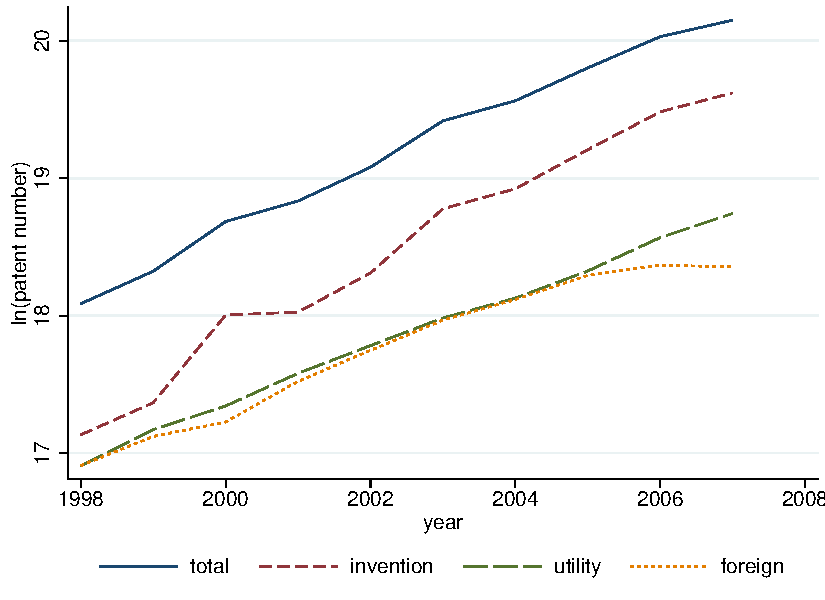
\includegraphics[width=\textwidth]{./figure/figure1.pdf}
\caption{\small Patent applications: 1998-2007}
\end{figure}
\clearpage



\def\sym#1{\ifmmode^{#1}\else\(^{#1}\)\fi}
\begin{table}[!h]
\caption{Descriptive Statistics}
\setlength{\abovecaptionskip}{0pt}
\setlength{\belowcaptionskip}{0pt}
{\tiny {
\resizebox{\textwidth}{!}{
\begin{tabular}{lccccc} \hline
Variable & Obs & Mean & Std.Dev. & Min & Max \\ \hline
lntfp & 1,110,681 & 2.555 & 1.227 & -11.41 & 15.22 \\
up\_spillover &  &  & &  &  \\
total patent number,direct & 1,110,681 & 5.504 & 0.786 & 1.378 & 8.020 \\
invention patent number,direct & 1,110,681 & 4.982 & 0.776 & 1.185 & 7.633 \\
citation,direct & 1,110,681 & 5.551 & 0.760 & 1.431 & 7.860 \\
total patent number,full-chain & 1,110,681 & 23.93 & 3.088 & 7.860 & 33.01 \\
invention patent number,full-chain& 1,110,681 & 21.66 & 2.979 & 7.023 & 30.33 \\
citation,full-chain & 1,110,681 & 23.97 & 2.763 & 8.536 & 31.82 \\
down\_spillover &  &  & &  &  \\
total patent number,direct & 1,110,681 & 5.889 & 2.817 & 0.528 & 10.99 \\
invention patent number,direct & 1,110,681 & 5.267 & 2.557 & 0.479 & 10.15 \\
citation,direct & 1,110,681 & 5.784 & 2.778 & 0.589 & 10.51 \\
total patent number,full-chain & 1,110,681 & 23.79 & 7.297 & 8.039 & 41.71 \\
invention patent number,full-chain & 1,110,681 & 21.40 & 6.864 & 7.154 & 39.08 \\
citation,full-chain & 1,110,681 & 23.46 & 7.476 & 8.608 & 41.54 \\
within-sector &  &  & &  &  \\
total patent number & 1,110,681 & 9.839 & 1.570 & 2.708 & 13.24 \\
invention patent number & 1,110,681 & 8.887 & 1.729 & 1.386 & 12.62 \\
citation & 1,110,681 & 9.704 & 1.676 & 1.609 & 13.08 \\
size & 1,110,681 & 10.26 & 1.270 & 0 & 19.04 \\
FinVuln & 1,091,273 & -0.0295 & 0.463 & -1.140 & 2.430 \\ \hline
\end{tabular}
}\\
}
}
\end{table}
\clearpage




\def\sym#1{\ifmmode^{#1}\else\(^{#1}\)\fi}
\begin{sidewaystable}[!h]
\caption{Vertical Spillovers and TFP:  Total application number}
\setlength{\abovecaptionskip}{0pt}
\setlength{\belowcaptionskip}{0pt}
{\tiny {
\resizebox{\textwidth}{!}{
\begin{tabular}{l*{8}{c}}
\hline\hline
            &\multicolumn{1}{c}{(1)}&\multicolumn{1}{c}{(2)}&\multicolumn{1}{c}{(3)}&\multicolumn{1}{c}{(4)}&\multicolumn{1}{c}{(5)}&\multicolumn{1}{c}{(6)}&\multicolumn{1}{c}{(7)}&\multicolumn{1}{c}{(8)}\\
            &\multicolumn{4}{c}{Direct}&\multicolumn{4}{c}{Full-chain}\\
\hline
up\_spillover  &  0.519\sym{**} &              & 0.476\sym{***}&    0.480\sym{***}&   0.133\sym{**} &              &0.112\sym{**} & 0.225\sym{***} \\
               &     (0.198)    &              &     (0.165)   &    (0.158)       &   (0.056)       &              &(0.050)       & (0.081)         \\
down\_spillover&                &  0.171\sym{*}&  0.149\sym{*} &    0.001         &                 &  0.054\sym{*}&  0.036       &  0.000          \\
               &                &     (0.093)  &     (0.076)   &   (0.088)        &                 &   (0.030)    &    (0.024)   &  (0.033)        \\
patent number     &          &                     &                     &      -0.031         &                     &                    &                     &      -0.214\sym{*}  \\
            &         &                     &                     &     (0.049)         &                     &                     &                     &     (0.110)         \\
size        &       &                     &                     &       0.723\sym{***}&                     &                     &                     &       0.724\sym{***}\\
            &        &                     &                     &     (0.005)         &                     &                     &                     &     (0.005)         \\
1=foreign   &      &                     &                     &      -0.018\sym{***}&                     &                     &                     &      -0.018\sym{***}\\
            &      &                     &                     &     (0.005)         &                     &                     &                     &     (0.006)         \\
firm fixed effects      &     yes         &       yes&     yes     &      yes&      yes        &     yes&    yes     &     yes\\
sector fixed effects      &     yes         &       yes&     yes     &      yes&      yes        &     yes&    yes     &     yes\\
year fixed effects      &     yes         &       yes&     yes     &      yes&      yes        &     yes&    yes     &     yes\\

\hline
\(N\)       &     1110681         &     1110681         &     1110681         &     1110681         &     1110681         &     1110681         &     1110681         &     1110681         \\
\(R^{2}\)   &       0.062         &       0.061         &       0.062         &       0.410         &       0.062         &       0.061         &       0.062         &       0.411         \\
\hline\hline
\end{tabular}
}\\
}
}
\scriptsize {
\par \emph{Notes}: Standard errors are clustered at sector level in parentheses. $^{***}$, $^{**}$ and $^{*}$ donate significance at the 1, 5 and 10\% level respectively. $up\_spillover$($down\_spillover$) is weighted average of $\ln$ total patent number from upstream(downstream). $size$ is $\ln$ firm total output. $1=foreign$ is an indicator variable equals one for foreign firm. $patent~number$ is the sum of patent applications number within sector.}
\end{sidewaystable}
\clearpage



\def\sym#1{\ifmmode^{#1}\else\(^{#1}\)\fi}
\begin{sidewaystable}[!h]
\caption{Vertical Spillovers and TFP: Citation}
\setlength{\abovecaptionskip}{0pt}
\setlength{\belowcaptionskip}{0pt}
{\tiny {
\resizebox{\textwidth}{!}{
\begin{tabular}{l*{8}{c}}
\hline\hline
            &\multicolumn{1}{c}{(1)}&\multicolumn{1}{c}{(2)}&\multicolumn{1}{c}{(3)}&\multicolumn{1}{c}{(4)}&\multicolumn{1}{c}{(5)}&\multicolumn{1}{c}{(6)}&\multicolumn{1}{c}{(7)}&\multicolumn{1}{c}{(8)}\\
            &\multicolumn{4}{c}{Direct}&\multicolumn{4}{c}{Full-chain}\\
\hline
up\_spillover  &  0.207         &              &       0.164   &     0.204\sym{*} &      0.020      &   & 0.010      & 0.172\sym{*}    \\
               &    (0.140)     &              &     (0.120)   &     (0.118)      &      (0.027)            &   &      (0.036)       & (0.089)         \\
down\_spillover&                &  0.156         &       0.127         &      -0.001      &                 &   0.019         &       0.014         &      -0.010          \\
               &                &     (0.113)  &        (0.100)        &      (0.114)     &                 &    (0.023)         &     (0.031)         &     (0.046)         \\
citation number   &                     &                     &                     &      -0.073\sym{*}  &                     &                     &                     &      -0.229         \\
            &                     &                     &                     &     (0.037)         &                     &                     &                     &     (0.139)         \\
size        &                     &                     &                     &       0.723\sym{***}&                     &                     &                     &       0.723\sym{***}\\
            &                     &                     &                     &     (0.005)         &                     &                     &                     &     (0.005)         \\
1=foreign   &                     &                     &                     &      -0.018\sym{***}&                     &                     &                     &      -0.018\sym{***}\\
            &                     &                     &                     &     (0.005)         &                     &                     &                     &     (0.005)         \\
firm fixed effects      &     yes         &       yes&     yes     &      yes&      yes        &     yes&    yes     &     yes\\
sector fixed effects      &     yes         &       yes&     yes     &      yes&      yes        &     yes&    yes     &     yes\\
year fixed effects      &     yes         &       yes&     yes     &      yes&      yes        &     yes&    yes     &     yes\\

\hline
\(N\)       &     1110681         &     1110681         &     1110681         &     1110681         &     1110681         &     1110681         &     1110681         &     1110681         \\
\(R^{2}\)   &       0.061         &       0.061         &       0.061         &       0.409         &       0.060         &       0.060         &       0.060         &       0.410         \\
\hline\hline
\end{tabular}
}\\
}
}
\scriptsize {
\par \emph{Notes}: Standard errors are clustered at sector level in parentheses. $^{***}$, $^{**}$ and $^{*}$ donate significance at the 1, 5 and 10\% level respectively. $up\_spillover$($down\_spillover$) is weighted average of $\ln$ total citation number in 5-year cohort from upstream(downstream). $size$ is $\ln$ firm total output. $1=foreign$ is an indicator variable equals one for foreign firm. $citation~number$ is the sum of citation number in 5-year cohort within sector.}
\end{sidewaystable}
\clearpage



\def\sym#1{\ifmmode^{#1}\else\(^{#1}\)\fi}
\begin{table}[!h]
\caption{Vertical Spillovers, Credit Constraints and TFP: Total application number}
\setlength{\abovecaptionskip}{0pt}
\setlength{\belowcaptionskip}{0pt}
{\tiny {
\resizebox{\textwidth}{!}{
\begin{tabular}{l*{6}{c}}
\hline\hline
            &\multicolumn{1}{c}{(1)}&\multicolumn{1}{c}{(2)}&\multicolumn{1}{c}{(3)}&\multicolumn{1}{c}{(4)}&\multicolumn{1}{c}{(5)}&\multicolumn{1}{c}{(6)}\\
            &\multicolumn{3}{c}{Direct}&\multicolumn{3}{c}{Full-chain}\\
\hline
up\_spillover &   0.538\sym{***} &   0.520\sym{***}&   0.502\sym{***} &   0.264\sym{***} &   0.250\sym{***} &   0.256\sym{***} \\

           &    (0.188) &    (0.165) &    (0.160) &    (0.087) &    (0.081) &    (0.079) \\

down\_spillover &      0.008 &      0.020 &      0.021 &      0.006 &      0.008 &      0.010 \\

           &    (0.089) &    (0.088) &    (0.085) &    (0.034) &    (0.034) &    (0.033) \\
up\_spillover\#FinVuln &      0.115 &            &      0.069 &      0.031 &            &      0.055 \\

           &    (0.127) &            &    (0.169) &    (0.030) &            &    (0.072) \\

down\_spillover\#FinVuln &            &      0.247 &    0.529\sym{**} &            &      0.045 &     0.171\sym{*} \\

           &            &    (0.159) &    (0.243) &            &    (0.037) &    (0.086) \\

patent number &     -0.052 &     -0.074 &     -0.077 &   -0.279\sym{**} &   -0.277\sym{**} &   -0.295\sym{**} \\

           &    (0.053) &    (0.056) &    (0.056) &    (0.124) &    (0.123) &    (0.125) \\
patent number\#FinVuln &            &            &   -0.161\sym{**} &            &            &   -0.349\sym{**} \\

           &            &            &    (0.072) &            &            &    (0.142) \\
      size &   0.724\sym{***} &   0.724\sym{***} &   0.724\sym{***} &   0.725\sym{***} &   0.725\sym{***} &   0.725\sym{***} \\

           &    (0.005) &    (0.005) &    (0.005) &    (0.005) &    (0.005) &    (0.005) \\

 1=foreign &  -0.017\sym{***} &  -0.017\sym{***} &  -0.017\sym{***} &  -0.017\sym{***} &  -0.017\sym{***} &  -0.017\sym{***} \\

           &    (0.005) &    (0.005) &    (0.005) &    (0.005) &    (0.005) &    (0.006) \\
firm fixed effects      &     yes         &       yes&     yes     &      yes&      yes        &     yes\\
sector fixed effects      &     yes         &       yes&     yes     &      yes&      yes        &     yes\\
year fixed effects      &     yes         &       yes&     yes     &      yes&      yes        &     yes\\

\hline
\(N\)       &     1091273 &    1091273 &    1091273 &    1091273 &    1091273 &    1091273   \\
\(R^{2}\)   &       0.411 &      0.411 &      0.412 &      0.411 &      0.411 &      0.412    \\
\hline\hline
\end{tabular}
}\\
}
}
\scriptsize {
\par \emph{Notes}: Standard errors are clustered at sector level in parentheses. $^{***}$, $^{**}$ and $^{*}$ donate significance at the 1, 5 and 10\% level respectively. $up\_spillover$($down\_spillover$) is weighted average of $\ln$ total paten application number from upstream(downstream). $FinVuln$ is the share of capital expenditures not financed out of cash flows from operations. $size$ is $\ln$ firm total output. $1=foreign$ is an indicator variable equals one for foreign firm. $patent~ number$ is the sum of patent application number within sector.}
\end{table}
\clearpage




\def\sym#1{\ifmmode^{#1}\else\(^{#1}\)\fi}
\begin{table}[!h]
\caption{Vertical Spillovers, Credit Constraints and TFP: Citation}
\setlength{\abovecaptionskip}{0pt}
\setlength{\belowcaptionskip}{0pt}
{\tiny {
\resizebox{\textwidth}{!}{
\begin{tabular}{l*{6}{c}}
\hline\hline
            &\multicolumn{1}{c}{(1)}&\multicolumn{1}{c}{(2)}&\multicolumn{1}{c}{(3)}&\multicolumn{1}{c}{(4)}&\multicolumn{1}{c}{(5)}&\multicolumn{1}{c}{(6)}\\
            &\multicolumn{3}{c}{Direct}&\multicolumn{3}{c}{Full-chain}\\
\hline
up\_spillover &     0.243\sym{*} &     0.225\sym{*} &    0.274\sym{**} &    0.197\sym{**} &    0.185\sym{**} &    0.204\sym{**} \\

           &    (0.128) &    (0.116) &    (0.137) &    (0.089) &    (0.085) &    (0.084) \\

down\_spillover &      0.006 &      0.009 &      0.015 &     -0.006 &     -0.005 &      0.003 \\

           &    (0.116) &    (0.113) &    (0.110) &    (0.048) &    (0.047) &    (0.046) \\
up\_spillover\#FinVuln &      0.179 &            &      0.137 &      0.037 &            &      0.030 \\

           &    (0.201) &            &    (0.396) &    (0.040) &            &    (0.128) \\
down\_spillover\#FinVuln &            &      0.315 &     0.716* &            &      0.049 &    0.282\sym{**} \\

           &            &    (0.223) &    (0.375) &            &    (0.045) &    (0.136) \\

citation number &    -0.080\sym{*} &    -0.083\sym{*} &   -0.096\sym{**} &    -0.264\sym{*} &    -0.254\sym{*} &   -0.291\sym{**} \\

           &    (0.041) &    (0.042) &    (0.042) &    (0.147) &    (0.143) &    (0.138) \\
citation number\#FinVuln &            &            &     -0.211 &            &            &   -0.435\sym{**} \\

           &            &            &    (0.129) &            &            &    (0.205) \\

      size &   0.724\sym{***} &   0.724\sym{***} &   0.724\sym{***} &   0.724\sym{***} &   0.724\sym{***} &   0.724\sym{***} \\

           &    (0.005) &    (0.005) &    (0.005) &    (0.005) &    (0.005) &    (0.005) \\

 1=foreign &  -0.018\sym{***} &  -0.017\sym{***} &  -0.017\sym{***} &  -0.017\sym{***} &  -0.017\sym{***} &  -0.017\sym{***} \\

           &    (0.005) &    (0.005) &    (0.005) &    (0.005) &    (0.005) &    (0.005) \\
\hline
firm fixed effects      &     yes         &       yes&     yes     &      yes&      yes        &     yes\\
sector fixed effects      &     yes         &       yes&     yes     &      yes&      yes        &     yes\\
year fixed effects      &     yes         &       yes&     yes     &      yes&      yes        &     yes\\

\hline
\(N\)       &     1091273 &    1091273 &    1091273 &    1091273 &    1091273 &    1091273   \\
\(R^{2}\)   &       0.410 &      0.410 &      0.411 &      0.410 &      0.410 &      0.411    \\
\hline\hline
\end{tabular}
}\\
}
}
\scriptsize {
\par \emph{Notes}: Standard errors are clustered at sector level in parentheses. $^{***}$, $^{**}$ and $^{*}$ donate significance at the 1, 5 and 10\% level respectively. $up\_spillover$($down\_spillover$) is weighted average of $\ln$ total citation number from upstream(downstream). $FinVuln$ is the share of capital expenditures not financed out of cash flows from operations. $size$ is $\ln$ firm total output. $1=foreign$ is an indicator variable equals one for foreign firm. $citation~number$ is the sum of patent application number within sector.}
\end{table}
\clearpage







\def\sym#1{\ifmmode^{#1}\else\(^{#1}\)\fi}
\begin{table}[!h]
\caption{Robustness: Invention patent number}
\setlength{\abovecaptionskip}{0pt}
\setlength{\belowcaptionskip}{0pt}
{\tiny {
\resizebox{\textwidth}{!}{
\begin{tabular}{l*{4}{c}}
\hline\hline
            &\multicolumn{1}{c}{(1)}&\multicolumn{1}{c}{(2)}&\multicolumn{1}{c}{(3)}&\multicolumn{1}{c}{(4)}\\
            &\multicolumn{2}{c}{Direct}&\multicolumn{2}{c}{Full-chain}\\
\hline
up\_spillover &   0.299\sym{***} &   0.328\sym{***} &   0.151\sym{***} &   0.181\sym{***} \\

           &    (0.099) &    (0.113) &    (0.056) &    (0.058) \\

down\_spillover &      0.003 &      0.027 &      0.001 &      0.012 \\

           &    (0.072) &    (0.072) &    (0.027) &    (0.028) \\
up\_spillover\#FinVuln &            &      0.058 &            &      0.041 \\

           &            &    (0.152) &            &    (0.066) \\

down\_spillover\#FinVuln &            &    0.426\sym{**} &            &     0.148\sym{*} \\

           &            &    (0.208) &            &    (0.078) \\

patent number &     -0.028 &     -0.049 &    -0.160\sym{*} &   -0.219\sym{**} \\

           &    (0.030) &    (0.035) &    (0.089) &    (0.097) \\

patent number\#FinVuln &            &   -0.138\sym{**} &            &   -0.294\sym{**} \\

           &            &    (0.064) &            &    (0.124) \\

      size &   0.723\sym{***} &   0.724\sym{***} &   0.724\sym{***} &   0.725\sym{***} \\

           &    (0.005) &    (0.005) &    (0.005) &    (0.005) \\

 1=foreign &  -0.018\sym{***} &  -0.017\sym{***} &  -0.018\sym{***} &  -0.017\sym{***} \\

           &    (0.005) &    (0.005) &    (0.005) &    (0.005) \\

           \hline
firm fixed effects      &     yes         &       yes&     yes     &      yes\\
sector fixed effects      &     yes         &       yes&     yes     &      yes\\
year fixed effects      &     yes         &       yes&     yes     &      yes\\
\hline
\(N\)       &     1110681 &    1091273 &    1110681 &    1091273 \\
\(R^{2}\)    &0.410 &      0.411 &      0.410 &      0.412 \\
\hline\hline
\end{tabular}
}\\
}
}
\scriptsize {
\par \emph{Notes}: Standard errors are clustered at sector level in parentheses. $^{***}$, $^{**}$ and $^{*}$ donate significance at the 1, 5 and 10\% level respectively. $up\_spillover$($down\_spillover$) is weighted average of $\ln$ invention patent number from upstream(downstream). $FinVuln$ is the share of capital expenditures not financed out of cash flows from operations. $size$ is $\ln$ firm total output. $1=foreign$ is an indicator variable equals one for foreign firm. $patent~number$ is the sum of invention patent applications number within sector.}
\end{table}
\clearpage



\def\sym#1{\ifmmode^{#1}\else\(^{#1}\)\fi}
\begin{table}[!h]
\caption{Robustness: Firm type}
\setlength{\abovecaptionskip}{0pt}
\setlength{\belowcaptionskip}{0pt}
{\tiny {
\resizebox{\textwidth}{!}{
\begin{tabular}{l*{4}{c}}
\hline\hline
            &\multicolumn{1}{c}{(1)}&\multicolumn{1}{c}{(2)}&\multicolumn{1}{c}{(3)}&\multicolumn{1}{c}{(4)}\\
            &\multicolumn{1}{c}{Private}&\multicolumn{1}{c}{Foreign}&\multicolumn{1}{c}{Private}&\multicolumn{1}{c}{Foreign}\\
\hline

up\_spillover &     0.175* &      0.153 &    0.187** &   0.247*** \\

           &    (0.090) &    (0.093) &    (0.081) &    (0.092) \\

down\_spillover &     -0.019 &      0.012 &      0.003 &      0.007 \\

           &    (0.045) &    (0.054) &    (0.047) &    (0.050) \\
up\_spillover\#FinVuln &            &            &     -0.002 &      0.154 \\

           &            &            &    (0.126) &    (0.125) \\

down\_spillover\#FinVuln &            &            &    0.323** &      0.143 \\

           &            &            &    (0.151) &    (0.104) \\

citation number &     -0.223 &     -0.223 &   -0.272** &   -0.332** \\

           &    (0.138) &    (0.157) &    (0.136) &    (0.151) \\
citation number\#FinVuln &            &            &   -0.432** &   -0.471** \\

           &            &            &    (0.212) &    (0.216) \\

size &   0.726*** &   0.721*** &   0.728*** &   0.721*** \\

           &    (0.006) &    (0.007) &    (0.006) &    (0.007) \\
           \hline
firm fixed effects      &     yes         &       yes&     yes     &      yes\\
sector fixed effects      &     yes         &       yes&     yes     &      yes\\
year fixed effects      &     yes         &       yes&     yes     &      yes\\
\hline
\(N\)       &     878541 &    232140 &    861871 &    229402 \\
\(R^{2}\)    &0.428 &      0.352 &      0.429 &      0.353 \\
\hline\hline
\end{tabular}
}\\
}
}
\scriptsize {
\par \emph{Notes}: Standard errors are clustered at sector level in parentheses. $^{***}$, $^{**}$ and $^{*}$ donate significance at the 1, 5 and 10\% level respectively. $up\_spillover$($down\_spillover$) is weighted average of $\ln$ total citation number from upstream(downstream). $FinVuln$ is the share of capital expenditures not financed out of cash flows from operations. $size$ is $\ln$ firm total output. $1=foreign$ is an indicator variable equals one for foreign firm. $citation~number$ is the sum of invention patent applications number within sector.}
\end{table}
\clearpage


\def\sym#1{\ifmmode^{#1}\else\(^{#1}\)\fi}
\begin{table}[!h]
\caption{Robustness: Initial firm size \& tfp }
\setlength{\abovecaptionskip}{0pt}
\setlength{\belowcaptionskip}{0pt}
{\tiny {
\resizebox{\textwidth}{!}{
\begin{tabular}{l*{4}{c}}
\hline\hline
            &\multicolumn{1}{c}{(1)}&\multicolumn{1}{c}{(2)}&\multicolumn{1}{c}{(3)}&\multicolumn{1}{c}{(4)}\\
            &\multicolumn{1}{c}{size}&\multicolumn{1}{c}{tfp}&\multicolumn{1}{c}{size}&\multicolumn{1}{c}{tfp}\\
\hline
up\_spillover &      0.177 &    0.297** &   0.281*** &   0.282*** \\

           &    (0.145) &    (0.142) &    (0.096) &    (0.096) \\

down\_spillover &     -0.001 &      0.013 &     -0.000 &      0.034 \\

           &    (0.049) &    (0.048) &    (0.046) &    (0.046) \\

up\_spillover\#rank &     -0.008 &  -0.238*** &            &            \\

           &    (0.006) &    (0.017) &            &            \\

down\_spillover\#rank &   -0.006** &  -0.030*** &    -0.005* &  -0.069*** \\

           &    (0.002) &    (0.005) &    (0.002) &    (0.005) \\

up\_spillover\#FinVuln &            &            &      0.280 &      0.283 \\

           &            &            &    (0.186) &    (0.185) \\

down\_spillover\#FinVuln &            &            &      0.154 &      0.158 \\

           &            &            &    (0.130) &    (0.132) \\
down\_spillover\#FinVuln\#rank &            &            &      0.005 &     -0.014 \\

           &            &            &    (0.003) &    (0.011) \\
citation number &     -0.195 &     -0.191 &   -0.344** &   -0.345** \\

           &    (0.186) &    (0.184) &    (0.146) &    (0.146) \\

citation\#FinVuln &            &            &  -0.756*** &   -0.753** \\

           &            &            &    (0.285) &    (0.284) \\



      size &   0.659*** &   0.648*** &   0.659*** &   0.656*** \\

           &    (0.008) &    (0.008) &    (0.008) &    (0.008) \\

 1=foreign &    -0.020* &    -0.018* &    -0.019* &    -0.019* \\

           &    (0.010) &    (0.010) &    (0.011) &    (0.011) \\



           \hline
firm fixed effects      &     yes         &       yes&     yes     &      yes\\
sector fixed effects      &     yes         &       yes&     yes     &      yes\\
year fixed effects      &     yes         &       yes&     yes     &      yes\\
\hline
\(N\)       &     216091 &     216091 &     212460 &     212460 \\
\(R^{2}\)   &     0.379  &      0.397 &      0.383 &      0.388     \\
\hline\hline
\end{tabular}
}\\
}
}
\scriptsize {
\par \emph{Notes}: Standard errors are clustered at sector level in parentheses. $^{***}$, $^{**}$ and $^{*}$ donate significance at the 1, 5 and 10\% level respectively. $up\_spillover$($down\_spillover$) is weighted average of $\ln$ total citation number from upstream(downstream). $FinVuln$ is the share of capital expenditures not financed out of cash flows from operations. $size$ is $\ln$ firm total output. $1=foreign$ is an indicator variable equals one for foreign firm. $citation~number$ is the sum of invention patent applications number within sector.}
\end{table}
\clearpage



\def\sym#1{\ifmmode^{#1}\else\(^{#1}\)\fi}
\begin{table}[!h]
\caption{Vertical Spillovers and TFP: Sector heterogeneity}
\setlength{\abovecaptionskip}{0pt}
\setlength{\belowcaptionskip}{0pt}
{\tiny {
\resizebox{\textwidth}{!}{
\begin{tabular}{l*{6}{c}}
\hline\hline
            &\multicolumn{1}{c}{(1)}&\multicolumn{1}{c}{(2)}&\multicolumn{1}{c}{(3)}&\multicolumn{1}{c}{(4)}&\multicolumn{1}{c}{(5)}&\multicolumn{1}{c}{(6)}\\
            &\multicolumn{1}{c}{Top 25\%}&\multicolumn{1}{c}{25\%-50\%}&\multicolumn{1}{c}{50\%-75\%}&\multicolumn{1}{c}{Bottom 25\%}&\multicolumn{1}{c}{High-tech}&\multicolumn{1}{c}{Low-tech}\\
\hline
up\_spillover &  -0.331*** &      0.282 &      0.027 &     0.177* &   0.661*** &      0.097 \\

           &    (0.107) &    (0.216) &    (0.066) &    (0.096) &    (0.124) &    (0.062) \\

down\_spillover &     -0.050 &     0.438* &     -0.003 &      0.035 &    0.206** &     -0.039 \\

           &    (0.043) &    (0.224) &    (0.099) &    (0.335) &    (0.086) &    (0.043) \\

citation number &   0.389*** &    -0.965* &     -0.040 &     -0.318 &  -1.110*** &-0.119 \\

           &    (0.135) &    (0.470) &    (0.157) &    (0.373) &    (0.147) &    (0.105) \\

      size &   0.722*** &   0.730*** &   0.750*** &   0.725*** &   0.721*** &   0.726*** \\

           &    (0.009) &    (0.016) &    (0.009) &    (0.008) &    (0.014) &    (0.005) \\

 1=foreign &    -0.018* &    -0.033* &   -0.025** &     -0.009 &      0.006 &  -0.021*** \\

           &    (0.009) &    (0.017) &    (0.009) &    (0.008) &    (0.013) &    (0.006) \\
firm fixed effects      &     yes         &       yes&     yes     &      yes&      yes        &     yes\\
sector fixed effects      &     yes         &       yes&     yes     &      yes&      yes        &     yes\\
year fixed effects      &     yes         &       yes&     yes     &      yes&      yes        &     yes\\

\hline
\(N\)       &     269662 &     280290 &     256932 &     303797 &      98921 &     997020     \\
\(R^{2}\)   &      0.349 &      0.420 &      0.422 &      0.394 &      0.461 &      0.401     \\
\hline\hline
\end{tabular}
}\\
}
}
\scriptsize {
\par \emph{Notes}: Standard errors are clustered at sector level in parentheses. $^{***}$, $^{**}$ and $^{*}$ donate significance at the 1, 5 and 10\% level respectively. $up\_spillover$($down\_spillover$) is weighted average of $\ln$ total citation number in 5-year cohort from upstream(downstream). $size$ is $\ln$ firm total output. $1=foreign$ is an indicator variable equals one for foreign firm. $citation~number$ is the sum of citation number in 5-year cohort within sector.}
\end{table}
\clearpage















\end{CJK*}
\end{document}
